\documentclass{article}

% use Times
\usepackage{times}
% For figures
\usepackage{graphicx} % more modern
%\usepackage{subfigure} 
\usepackage{subcaption}


% For citations
\usepackage{natbib}

% For algorithms
\usepackage{algorithm}
\usepackage{algorithmic}

% As of 2011, we use the hyperref package to produce hyperlinks in the
% resulting PDF.  If this breaks your system, please commend out the
% following usepackage line and replace \usepackage{icml2016} with
% \usepackage[nohyperref]{icml2016} above.
\usepackage{hyperref}

% Packages hyperref and algorithmic misbehave sometimes.  We can fix
% this with the following command.
\newcommand{\theHalgorithm}{\arabic{algorithm}}

% Employ the following version of the ``usepackage'' statement for
% submitting the draft version of the paper for review.  This will set
% the note in the first column to ``Under review.  Do not distribute.''
\usepackage{icml2016} 
\usepackage{amsmath,amsfonts,amssymb}
\usepackage{dsfont}
\usepackage{booktabs}
\usepackage{relsize}
\usepackage{lmodern}
\usepackage{slantsc}
\usepackage{siunitx}
\sisetup{output-exponent-marker=\ensuremath{\mathrm{E}}}


\newcommand{\xsj}{\mathbf{\hat{x}}_j}
\newcommand{\xuj}{\mathbf{x}_j}
\newcommand{\xsi}{\mathbf{\hat{x}}_i}
\newcommand{\xui}{\mathbf{x}_i}
\newcommand{\ysi}{\hat{y}_i}
\newcommand{\ysj}{\hat{y}_j}
\newcommand{\yui}{y_i}
\newcommand{\sw}{s_{ \textsc{\relsize{-2}{\textsl{W}}} }}



% Employ this version of the ``usepackage'' statement after the paper has
% been accepted, when creating the final version.  This will set the
% note in the first column to ``Proceedings of the...''
%\usepackage[accepted]{icml2016}


% The \icmltitle you define below is probably too long as a header.
% Therefore, a short form for the running title is supplied here:
\icmltitlerunning{Transductive Unsupervised Domain Adaptation}

\begin{document} 

\twocolumn[
\icmltitle{Transductive Unsupervised Domain Adaptation}

% It is OKAY to include author information, even for blind
% submissions: the style file will automatically remove it for you
% unless you've provided the [accepted] option to the icml2016
% package.
\icmlauthor{Ozan Sener}{ozansener@cs.stanford.edu}
\icmladdress{Stanford University,
		     Stanford, CA 94304, USA}
		     \vspace{-2mm}
\icmladdress{Cornell University,
		     Ithaca, NY 14853, USA}
\icmlauthor{Hyun Oh Song}{hsong@cs.stanford.edu}
\icmladdress{Stanford University,
		     Stanford, CA 94304, USA}

\icmlauthor{Silvio Savarese}{ssilvio@stanford.edu}
\icmladdress{Stanford University,
		     Stanford, CA 94304, USA}
\icmlauthor{Ashutosh Saxena}{ashutosh@brainoft.com}
\icmladdress{Brain of Things,
		     Cupertino, CA 94304, USA}


% You may provide any keywords that you 
% find helpful for describing your paper; these are used to populate 
% the "keywords" metadata in the PDF but will not be shown in the document
\icmlkeywords{domain adaptation, transductive learning, metric learning, deep learning}

\vskip 0.3in
]

\begin{abstract} 
Lorem ipsum dolor sit amet, consectetur adipiscing elit. Ut porta diam sit amet diam eleifend, eget pulvinar nunc ultrices. Phasellus elementum eros lorem, id dapibus sem accumsan ac. Fusce accumsan erat tincidunt arcu vestibulum auctor. Integer sit amet aliquam ipsum. Curabitur pellentesque finibus urna nec laoreet. Ut cursus dolor nisl, vitae molestie sem venenatis sit amet. Praesent non neque augue. Pellentesque libero diam, congue non neque non, blandit vehicula justo. Donec ultricies sed turpis quis condimentum. Nunc consequat metus ut nisi euismod, et venenatis ipsum elementum. Cras congue eleifend pulvinar. Cras eu eros sed nunc feugiat lobortis vel id mi. Pellentesque finibus turpis quis nisl tristique, sit amet vestibulum risus vehicula. Morbi quis cursus purus, id sodales felis.
\end{abstract} 

\section{Introduction}
\label{intro}


Recently deep convolutional neural networks \cite{alexnet, vggnet, googlenet} have propelled unprecedented advances in artificial intelligence including object recognition, speech recognition, and image captioning. However, one of the major drawbacks of the method is that the network requires a lot of labelled training data to fit millions of parameters in the complex network model. However, creating such datasets with complete annotations is not only tedious and error prone but also extremely costly. In this regard, the research community have proposed different mechanisms such as semi-supervised learning \cite{semisup1,semisup2,semisup3}, transfer learning \cite{transfer1, transfer2}, weakly labelled learning, and domain adaptation techniques. Of the approaches, domain adaptation is one of the most appealing technique when a fully annotated dataset (i.e. ImageNet \cite{ImageNet}, Sports1M \cite{sports1m}) is available as a reference. 

Formally, the goal of unsupervised domain adaptation is; given a fully supervised source dataset and a unsupervised target dataset, learning a model which can generalize to target domain while taking the domain shift across the datasets into account. The majority of the literature \cite{gong12, baochen15, fernando13, baochen16, tommasi13} in unsupervised domain adaptation formulates a learning problem where the task is to find a transformation matrix to align the labelled source data distribution to unlabelled target data distribution. Although these approaches show promising results, it does not take the actual inference procedure into the learning algorithm.

Concretely, we formulate a unified framework where the domain transformation parameter and the target labels are jointly optimized in two alternating stages. In the transduction stage, given a fixed domain transform parameter, we jointly infer all target labels by solving a discrete multi-label energy minimization problem. In the adaptation stage, given a fixed target label assignment, we seek to find the optimal asymmetric metric transformation between the source and the target data. The advantage of the method is that the we can learn a domain transformation parameter which is aware of the subsequent transductive inference procedure. 

Following the standard evaluation protocol in the domain adaptation community, we evaluate our method on the digit classification task using MNIST \cite{mnist} and SVHN\cite{svhn} as well as the object recognition task using the Office \cite{office} dataset, and demonstrate state of the art performance in comparison to all existing unsupervised domain adaptation methods.

\section{Related Work} 

This paper is closely related to two active research areas: (1) Unsupervised domain adaptation, and (2) Transductive learning.

\textbf{Unsupervised domain adaptation}: \cite{gong12, baochen15, fernando13, baochen16} proposed subspace alignment based approaches to unsupervised domain adaptation where the task is to learn a joint transformation and projection where the difference between the source and the target covariance is minimized. However, these method learn the transform matrices on the whole source and target dataset without utilizing the the source labels. 

\cite{tommasi13} utilizes local max margin metric learning objective \cite{lmnn} to first assign the target labels with nearest neighbor scheme and then learn a distance metric to enforce that the negative pairwise distances are larger than the positive pairwise distances with a margin. However, this method learns a symmetric distance matrix shared by both the source and the target domains so the method is susceptible to the discrepancies between the source and the target distributions. Recently, \cite{ganin15, tzeng14} proposed a deep learning based method to learn domain invariant features via providing the reversed gradient signal from the binary domain classifiers. Although they perform better than aforementioned approaches, their accuracy is limited since domain invariance do not necessarily imply discriminative features in the target domain. In other words, they seek for invariance instead of an equivariance. 

\textbf{Transductive learning}: In transductive learning literature \cite{transduction}, the model has access to unlabelled test samples during training. Recently, \cite{coclassification} tackled a classification problem where predictions are made jointly across all test examples in a transductive \cite{transduction} setting. The method essentially enforces the notion that the true labels vary smoothly with respect to the input data. In our work, we extend this notion to infer the multiclass labels of unsupervised target data in a k-NN graph. 

To summarize, our main contribution is to formulate joint optimization framework where we alternate between inferring target labels via discrete energy minimization (\textit{transduction}) and learning asymmetric transformation (\textit{adaptation}) between source and target examples. Our experiments on digit classification using MNIST \cite{mnist} and SVHN\cite{svhn} as well as the object recognition experiments on Office \cite{office} datasets show state of the art results outperforming all existing methods by a substantial margin.


\section{Method} 
% !TEX root = domain_transduction.tex
%We address the problem of unsupervised transductive domain adaptation by jointly solving for the label assignment of unsupervised target domain as well as the shift domain shift in the following subsections. %We first define our model in Section~\ref{prob:def} and explain the two sub-problems of transduction and adaptation. We further explain the details of transduction in Section~\ref{label} and the details of adaptation in Section~\ref{metric}.
%Unsupervised domain adaptation is inherently a transduction problem since the main challenge lies in labeling the unsupervised data points with the help of the supervised data; because, adaptation is done offline without computationally concerns and the accuracy is critical since the transduction error is a good proxy for generalization \cite{adapttheory}. Main complication, which makes existing transduction methods inapplicable, is the domain shift between the supervised and unsupervised data points . We explicitly model the domain shift and jointly solve for unsupervised labels as well as the domain shift in a transductive learning setup.

\subsection{Problem Definition and Notation}
\label{prob:def}
In unsupervised domain adaptation problem, one of the domains (source) is supervised $\{\xsi, \ysi \}_{i \in [N^s]}$ with $N^s$ data points $\xsi$ and corresponding labels $\ysi$ from a discrete set $\ysi \in \mathcal{Y} = \{1,\ldots, Y \}$.  The other domain (target), on the other hand is unsupervised and has $N^u$ data points $\{\xui \}_{i \in [N^u]}$. 

We further assume that both domains have different distributions $\xsi \sim p_s$ and $\xui \sim p_t$ defined on the same space as $\xsi,\xui \in \mathcal{X}$. We consider a case in which there are two feature functions  \mbox{$\Phi_s, \Phi_t:\mathcal{X}\rightarrow \mathcal{R}^d$} applicable to source and target separately. These feature functions extracts both the information shared among domains and explicit to the individual ones. The way we model common features is by sharing a subset of parameters between feature functions as \mbox{$\Phi_s=\Phi_{\theta_c,\theta_s}$} and \mbox{$\Phi_t=\Phi_{\theta_c,\theta_t}$}. We use deep neural networks to implement these functions and in our implementation $\theta_c$ corresponds to the parameters in the first few layers of the networks and $\theta_s$, $\theta_t$ corresponds to the respective final layers. In general, our model is applicable any hierarchical and differentiable feature function which can be expressed as a composite function $\Phi_s = f_{\theta_s}(g_{\theta_c}(\cdot))$ for source and similarly for target.

\subsection{Consistent Structured Transduction}
% talk about cyclic consistency and structured consistency
Our method is based on jointly learning the transferable domain specific representations for source and target points as well as estimating the labels of the unsupervised data-points. We denote these two main components of our method as transduction and adaptation. The transduction is the sub-problem of labelling unsupervised data points and the adaptation is solving for the domain shift. In order to solve this joint problem tractably, we exploit two heuristics; cyclic consistency for transduction and structured consistency for adaptation. 

\textbf{Cyclic consistency:} One desired property of  $\Phi_s$ and $\Phi_t$ is their consistency. If we estimate the labels of the unsupervised data points and further use these points to estimate the labels of supervised data-points, we want the predicted labels of the supervised data-points to be consistent with the ground truth labels. Using inner product as an asymmetric similarity metric -$s(\xsi, \xuj) = \Phi_s(\xsi)^\intercal \Phi_t(\xuj)$-,

\begin{displaymath}
    \xymatrix{
        (\xsi,\ysi) \ar@{<-}@<-2pt>`d[r] `[rrrrrr]|{\textbf{Cyclic Consistency: $\ysi = \ysi^{pred}$}} [rrrrrr]  \ar[rrr]|{\textbf{Transduction}}     &&& (\xuj, \yuj) \ar[rrr]|{\textbf{Transduction}} &&&  (\xsi,\ysi^{pred}) }
\end{displaymath}

It can be shown that; if the transduction from target to source follows a nearest neighbor rule, cyclic consistency can be enforced without explicitly computing $\ysi^{pred}$ using the large-margin nearest neighbor (LMNN)\cite{lmnn} rule. For each source point, we enforce a margin between its similarity with the nearest neighbor from the target having the same label and having a different label as; $ \Phi_s(\xsi)^\intercal \Phi_t(\mathbf{x}_{i^+}) > \Phi_s(\xsi)^\intercal \Phi_t(\mathbf{x}_{i^-}) + \alpha$ where $\mathbf{x}_{i^+}$ is the nearest target having the same class label as $\xsi$ and $\mathbf{x}_{i^-}$ is the nearest target having a different class label. 


\textbf{Structured consistency:} We enforce a structured consistency when we label the target data-points during the transduction. In other words, if two target data-points are similar to each other, they are more likely to have same label. To enforce this consistency, we create a k-NN graph of target data points using a similarity metric $\Phi_t(\xui)^\intercal \Phi_t(\xuj)$. We denote the neighbors of the point $\xsi$ as $\mathcal{N}(\xsi)$. We enforce structured consistency by penalizing neighbor points of same labels with their similarity score. 

Our model leads to the following optimization problem, over the target labels $\yui$ and the feature function parameters $\theta_c, \theta_s, \theta_t$, jointly solving transduction and adaptation. 
\begin{equation}
\small
\begin{aligned}
\min_{\substack{\theta_c,\theta_s,\theta_t, \\ y_1, \ldots y_{N^u}}} &\underbrace{\sum_{i \in [N^s]} [\Phi_s(\xsi)^\intercal \Phi_t(\mathbf{x}_{i^-}) -\Phi_s(\xsi)^\intercal \Phi_t(\mathbf{x}_{i^+}) + \alpha]_{+}}_{\text{Cyclic Consistency}}  +\underbrace{\lambda \sum_{i \in [N^u]} \sum_{\xuj \in \mathcal{N}(\xui)}  \Phi_t(\xui)^\intercal \Phi_t(\xuj) \mathds{1}(y_i \neq y_j)}_{\text{Structured Consistency}}\\
% \Phi(\xui)^\intercal \Phi(\xuj) \mathds{1}(y_i \neq y_j)\\
s.t. &\quad i^{+} = {\arg\max}_{j | y_j = \hat{y}_i} \Phi_s(\xsi)^\intercal \Phi_t(\xuj) \quad \quad \text{and} \quad \quad  i^{-} = {\arg\max}_{j | y_j \neq \hat{y}_i}  \Phi_s(\xsi)^\intercal \Phi_t(\xuj)
\end{aligned}
\label{loss}
\end{equation}
where $\mathds{1}(a)$ is an indicator function which is $1$ if $a$ is true and $0$ otherwise. $[a]_+$ is a rectifier function which is equal to $\max(0, a)$.


We solve this optimization problem via alternating minimization through iterating over solving for unsupervised labels $y_i$(transduction) and learning the similarity metric $\theta_c,\theta_s,\theta_t$ (adaptation). We explain these two steps in detail in the following sections.


 %} $ 

%$\max_{y_1} \$
%$\min_{y_1} + 
%_4) $ assuming green is $0$, blue is $1$ and red is $2$

\subsection{Transduction: Labeling Target Domain}
\label{label}
In order to label the unsupervised points, we use the k-nearest-neighbor rule. We simply compute the k-NN supervised data point for each unsupervised data point using the learned metric and transfer the corresponding majority label. Formally, given a similarity metric $\theta_c, \theta_s, \theta_t$, the k-NN rule is 
$(y_i)^{pred} = \arg\max_y \frac{k_y(\xui)}{k}$ where $k_y(\xui)$ is the number of samples having label $y$ in the $k$ nearest neighbor of $\xui$ from the source domain. One major issue with this approach is the accuracy of transduction during the initial stage of the algorithm. Since the learned metric will not be accurate, we expect to see some noisy k-NN sets. Hence, we propose two solutions to solve this problem.

\textbf{Structured Consistency:} Similar to existing graph transduction algorithms \cite{label_prop1,label_prop2}, we create a k-nearest neighbor (k-NN) graph over the unsupervised data points and penalize disagreements of labels between neighbors.

\textbf{Reject option:} In the initial stage of the algorithm, we let the transduction step to use reject $R$ as an additional label (besides the class labels) to label the unsupervised target points. In other words, our transduction algorithm can decide to not label (reject) some of the points so that they will not be used for adaptation. When the learned metric gets more accurate in the future iterations, transduction algorithm can change the label from R to other class labels. We define our transduction sub-problem as:

\begin{equation}
\begin{aligned}
\min_{y_1, \ldots y_{N^u} \in \mathcal{Y} \cup R}  &\sum_{i \in [N^u]} l(\xui, y_i) + \lambda \sum_{i \in [N^u]} \sum_{\xuj \in \mathcal{N}(\xui)} \Phi_t(\xui)^\intercal \Phi_t(\xuj)\mathds{1}(y_i \neq y_j)
\end{aligned}
\label{robtran}
\end{equation}

where $l(\xui, y) = \left\{ \begin{array}{cc}  1 - \frac{k_y(\xui)}{k} & y \in \mathcal{Y} \\ \gamma \max_{y^\prime \in \mathcal{Y}} \frac{k_y^\prime(\xui)}{k}
 & y=R \end{array}\right.$ and $\gamma$ is relative cost of the reject option. 
 
The $l(\xui,R)$ is smaller if none of the class has a majority, promoting reject option for undecided cases. We also modulate the $\gamma$ during learning to decrease number of reject options in the later stage of the adaptation. This problem can approximately be solved using many existing methods. We use the $\alpha$-$\beta$ swapping algorithm from \cite{kolmogrovalphabeta} since it is experimentally shown to be efficient and accurate. %In order to further explain the label propagation, we visualize an example with $k=4$ and $4$-class classification problem in Figure~\ref{vis_label_prop}. 

\iffalse
\begin{wrapfigure}{r}{0.5\textwidth}
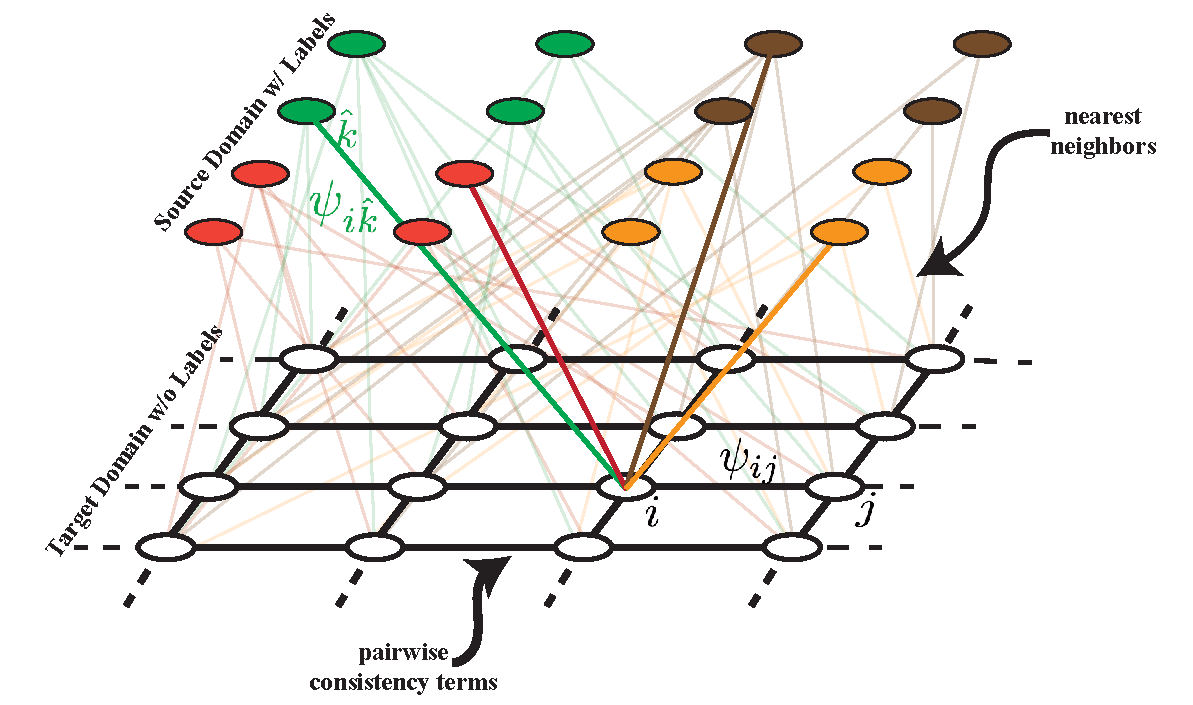
\includegraphics[width=0.5\textwidth]{fig11}
\caption{\textbf{Visualization of the Label Propogation.} We create a k-NN graph of unsupervised target points to enforce consistency with pairwise terms 
\mbox{$\psi_{ij}=sim(\mathbf{x}_i, \mathbf{x}_j) \mathds{1}(y_i \neq y_j)$} and use closest supervised source points to each class as 
\mbox{$ \psi_{i\hat{k}} \sw(\mathbf{\hat{x}}_k,\mathbf{x}_{i})$}.} 
\vspace{-1cm}
\label{vis_label_prop}
\end{wrapfigure}
\fi

\subsection{Adaptation: Learning the Metric}
\label{metric}
Given the predicted labels $y_i$ for unsupervised data points $\xui$, we can then learn a metric in order to minimize the loss function defined in (\ref{loss}). Following the cyclic consistency construction, the LMNN rule can be represented using the triplet loss defined between the supervised source data points and their nearest positive and negative neighbors among the unsupervised target points. We do not include the target-data points with reject label during this construction. Formally, we can define the adaptation problem given unsupervised labels as;
\begin{equation}
\begin{aligned}
\min_{\theta_c,\theta_s,\theta_t} &\sum_{i \in [N^s]} [\Phi_s(\xsi)^\intercal \Phi_t(\mathbf{x}_{i^-}) -\Phi_s(\xsi)^\intercal \Phi_t(\mathbf{x}_{i^+}) + \alpha]_{+} \\
\end{aligned}
\end{equation}
where 
\begin{equation}
i^{+} = {\arg\max}_{j | y_j = \hat{y}_i} \Phi_s(\xsi)^\intercal \Phi_t(\xuj) \quad  \text{and} \quad   i^{-} = {\arg\max}_{j | y_j \neq \hat{y}_i, y_j \neq R}  \Phi_s(\xsi)^\intercal \Phi_t(\xuj)
\label{sup_nn}
\end{equation}


%\begin{equation}
%\frac{\partial loss}{\partial \theta_s} = \sum_{i \in [N^s]} \mathds{1}(\Phi_s(\xsi)^\intercal \Phi_t(\mathbf{x}_{i^+}) - \Phi_s(\xsi)^\intercal \Phi_t(\mathbf{x}_{i^-}) < \alpha) \left[ \frac{\partial \Phi_s(\xsi)^\intercal}{\theta_s} \left(\Phi_t(\mathbf{x}_{i^+}) -  \Phi_t(\mathbf{x}_{i^-})\right) \right]
%\end{equation}
%\begin{equation}
%\frac{\partial loss}{\partial \theta_t} = 
%\sum_{i \in [N^s]} \mathds{1}(\Phi_s(\xsi)^\intercal \Phi_t(\mathbf{x}_{i^+}) - \Phi_s(\xsi)^\intercal \Phi_t(\mathbf{x}_{i^-}) < \alpha) \left[ \left(\frac{\partial \Phi_t(\mathbf{x}_{i^+})^\intercal}{\theta_t} - \frac{\partial \Phi_t(\mathbf{x}_{i^-})^\intercal}{\theta_t} \right)  \Phi_s(\xsi) \right]
%\end{equation}

This minimization is convex if feature functions are convex. This is typically not the case with convolution neural networks; however, the gradient descent type algorithms are still applicable and works well in practice. Hence, we optimize this function via stochastic gradient descent using the sub-gradients $\frac{\partial loss}{\partial \theta_s}, \frac{\partial loss}{\partial \theta_t}$ and $\frac{\partial loss}{\partial \theta_c}$. These sub-gradients can be efficiently computed with back-propagation \emph{(see supplementary material for details)}.


\subsection{Implementation Details}
\label{imp_det}
We use Alexnet~\cite{alexnet} and LeNet~\cite{lenet} architectures with small modifications. We remove their final softmax layer and change the size of the final fully connected layer according to the desired feature dimension. We consider the last fully connected layer as domain specific feature ($\theta_s$, $\theta_t$) and the rest as common network $\theta_c$. Common network weights are tied between domains, and the final layers are learned separately. In order to have a fair comparison with existing algorithms, we follow the same architecture used by \cite{ganin15} only modifying the final feature dimensionality (embedding size). Explicitly, we use the following architectures for domains:

\noindent \textbf{MNIST} and \textbf{SVHN:} LeNet\cite{lenet} as; 
\includegraphics[width=0.40\columnwidth]{lenet}

\noindent \textbf{Office:} AlexNet\cite{alexnet} as; 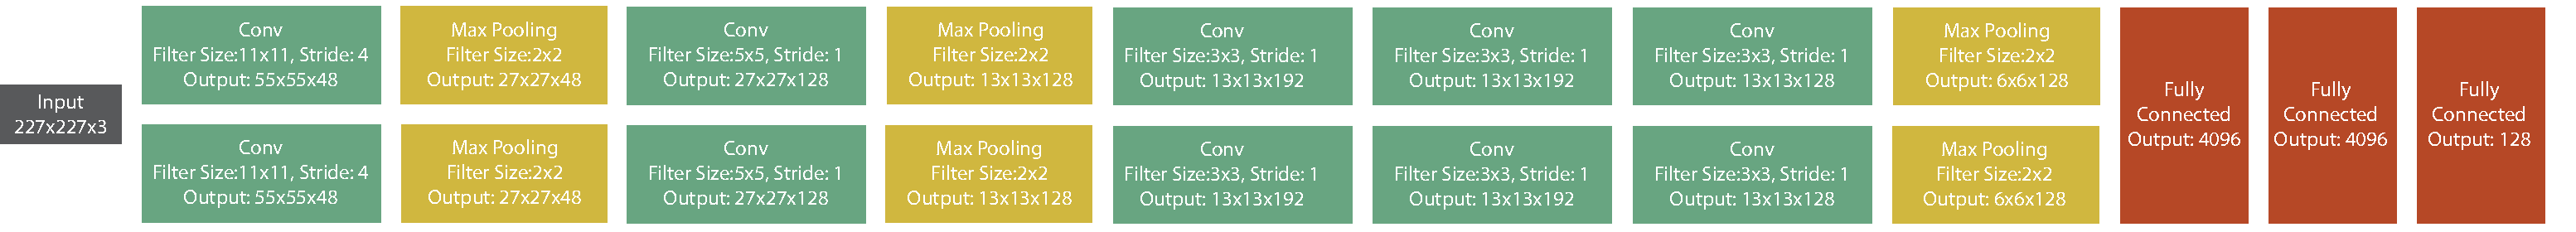
\includegraphics[width=0.73\columnwidth]{alexnet}

\begin{wrapfigure}{r}{0.5\textwidth}
    \begin{minipage}{0.5\textwidth}
    \vspace{-9mm}
\begin{algorithm}[H]
   \caption{Transduction with Domain Shift}
   \label{alg:example}
  \small
\begin{algorithmic}
   \STATE {\bfseries Input:} Source $\mathbf{\hat{x}}_{1 \cdots N^s},\hat{y}_{1, \cdots N^s}$, Target $\mathbf{x}_{1,\cdots,N^u}$, Batch Size $2\times B$
   \FOR  {$t=0$ \textbf{ to } \texttt{max\_iter} }
   \STATE  Sample $\{\xsb,\ysb \}$, $\{\xub\}$
   \STATE Solve (\ref{robtran}) for $\{y_{1 \cdots B}\}$
   \STATE $\alpha \leftarrow 0$
   \FOR{$i=1$ {\bfseries to} $B$}
      \IF{$ \hat{y}_i \in y_{1 \cdots B} \textbf{ and } \exists k ~y_k \in \mathcal{Y} /\hat{y}_i$} 
   \STATE Compute ($i^+, i^-$) using $\{y_{1 \cdots B}\}$ in (\ref{sup_nn})
   \STATE Update $\frac{\partial loss}{\partial \mathbf{\theta_c}}$,  $\frac{\partial loss}{\partial \mathbf{\theta_s}}$, $\frac{\partial loss}{\partial \mathbf{\theta_t}}$
   \STATE $\alpha \leftarrow \alpha + 1$
   \ENDIF
   \ENDFOR
   \IF{$\alpha > 0$}
   \STATE $\eta(t) \leftarrow$ Adagrad Rule \cite{adagrad}
   \STATE $\mathbf{\theta_c} \leftarrow \mathbf{\theta_c} + \eta(t) \frac{1}{\alpha} \frac{\partial loss}{\partial \mathbf{\theta_c}}$, $\mathbf{\theta_s} \leftarrow \mathbf{\theta_s} + \eta(t) \frac{1}{\alpha} \frac{\partial loss}{\partial \mathbf{\theta_s}}$, \\ $\mathbf{\theta_t} \leftarrow \mathbf{\theta_t} + \eta(t) \frac{1}{\alpha} \frac{\partial loss}{\partial \mathbf{\theta_t}}$
   \ENDIF
   \ENDFOR
\end{algorithmic}
\end{algorithm}
\vspace{-18mm}
  \end{minipage}
  \end{wrapfigure}
  
  where \textbf{C} is convolution, \textbf{P} is max-pooling, \textbf{R} is ReLU and \textbf{F} is fully connected layer. 


Since the office dataset is quite small, we do not learn the network from scratch for office experiments and instead we initialize with the weights pre-trained on ImageNet. In all of our experiments, we set the feature dimension as $128$. We use stochastic gradient descent to learn the feature function with AdaGrad\cite{adagrad}. We initialize variables with truncated normals having unit variance and use the learning rate \SI{2.5e-4}  and the batch size $512$. We start the rejection penalty with $\gamma=0.1$ and linearly increase with each epoch as $\gamma=\frac{\#epoch -1}{M}+0.1$. In our experiments we use $M=20$ and discuss the sensitivity of our algorithm to $M$ in supplementary material.
  


\section{Experimental Results}
% !TEX root = domain_transduction.tex
We evaluate our algorithm on various unsupervised domain adaptation tasks while focusing on two different problems, hand-written digit classification and object recognition. For each experiment, we use three domains and extensively evaluate all transfer scenarios.

\begin{table*}[ht]
\caption{Accuracy of our method and the state-of-the-art algorithms on Office dataset and various adaptation settings}
\label{tab:res}
\begin{sc}
\begin{center}
\begin{small}
\begin{tabular}{@{}rcccccc@{}} \toprule 
 Source & Amazon & D-SLR & Webcam & Webcam &Amazon & D-SLR \\
 Target & Webcam & Webcam & D-SLR & Amazon & D-SLR & Amazon \\
 \midrule
GFK \cite{gong2012} & $.398$ & $.791$ & $.746 $ & $.371$ & $.379$ & .379   \\
SA* \cite{fernando13} & $.450$ & $.648$ & $.699$ & $.393$ & $.388$ & $.420$ \\
DLID \cite{chopra13} & $.519$ & $.782$ & $.899$ & -&- &- \\
DDC \cite{tzeng14} & $.618$ & $.950$ & $.985$ & $.522$ & $.644$& $.521$\\
DAN \cite{wang15} & $.685$ & $.960$ & $.990$ & $.531$ & $.670$ & $.540$ \\
Backprop \cite{ganin15} & $.730$ &$\mathbf{.964}$ & $\mathbf{.992}$ & $.536$ & $.728$ & $.544$\\
\midrule
Source Only & $.642$ & $.961$ & $.978$ & $.452$ & $.668$ & $.476$ \\
Our Method & $\mathbf{.804}$ &.962 & $.989$ & $\mathbf{.625}$ & $\mathbf{.839}$ & $\mathbf{.567}$ \\
 \bottomrule
\end{tabular}
\end{small}
\end{center}
\end{sc}
\end{table*}

\begin{table}[ht]
\caption{Accuracy of our method and the digit classification task.}
\label{tab:res2}
\begin{sc}
\begin{small}
\resizebox{\columnwidth}{!}{%
\begin{tabular}{@{}r@{\hskip 1mm}c@{\hskip 1mm}c@{\hskip 1mm}c@{\hskip 1mm}c@{}} \toprule 
Source & M-M & MNIST  & SVHN & MNIST \\
Target&  MNIST & M-M & MNIST & SVHN\\
 \midrule
SA* \cite{fernando13}&  & $.569$ & $.593$ & \\
BP \cite{ganin15} &$.732$ & $.766$ & $.738$ & $.289$ \\
\midrule
Source Only  & $.483$ & $.522$  &.549 &\\
Our Method & $\mathbf{.835}$ & $\mathbf{.855}$ & $\mathbf{.774}$ & $\mathbf{.323}$\\
 \bottomrule
\end{tabular}}
\end{small}
\end{sc}
\end{table}
\subsection{Dataset}
In order to experiment our algorithm on the task of digit classification, we use MNIST\cite{mnist}, Street View House Number\cite{svhn} and artificailly generated version of MNIST which is MNIST-M\cite{ganin15}. MNIST-M is a simply a blend of the digit images of the original MNIST dataset and the color images of BSDS500\cite{bsds500} following the method explained in \cite{ganin15}. Since the dataset is not distributed directly by the authors, we generated the dataset using the same procedure and further confirmed that the performance is similar to the one reported in \cite{ganin15}. Street view house numbers dataset is a collection of house numbers collected directly from Google street view images. All these three domains are quite different from each other and among many important differences,most significant ones are MNIST being grayscale and the others being colored, and SVHN images having extra confusing digits around the centered digit of interest. Moreover, all three of these domains are large-scale having at least 60k examples over 10 classes. 

On the other hand, we use Office\cite{office} dataset in order to evaluate our algorithm on the task of object recognition. Office dataset includes images of the same objects taken directly from Amazon, captured with a low-resolution webcam and captured with a D-SLR camera. Notable differences of these domains include the white background of Amazon images vs realistic backgrounds of webcam and D-SLR images, and the resolution difference of webcam and D-SLR. Office dataset have rather fewer number of images as maximum 2478 images per domain. On the other hand, it has larger number of classes since there are 31 object categories.



\subsection{Baselines}
We compare our method with variety of algorithms both using and not using feature learning. Considering the two different lines of work, \textbf{SA*}\cite{fernando13} is the dominant state-of-the-art approach not employing any feature learning on other hand \textbf{Backprop(BP)}\cite{ganin15} is the dominant state-of-the-art approach employing feature learning. We use the available source code of \cite{ganin15} and \cite{fernando13} and following the evaluation procedure in \cite{ganin15}, we choose the hyper-parameter of \cite{fernando13} as the highest performing one among various alternatives. In addition to the baselines, we also compare our method with various self-baselines. The most important one is the \textbf{source only} baseline which is a convolutional neural network trained only using the source code. This classifier is clearly different from our nearest neighbor classifier; however, we experimentally validated that CNN always outperformed the nearest neighbor based classifier. Hence, we report the highest performing source only method in our results.

\subsection{Implementation Details}
\label{imp_det}
Although our algorithm have very few design parameters and we decide most of them either using cross-validation or exhaustive grid search, our algorithm uses an existing differentiable feature function. The selection of this feature function is a critical parameter for our algorithm. Following the unparalleled success of convolutional neural networks (CNNs), we use CNNs as our feature functions.  In order to have  fair comparison with existing algorithms, we follow the same architecture used by \cite{ganin15} by only changing the final feature dimensionality (embedding size). We use the following architectures for domains \emph{(see supplementary material for full details)}:

\noindent \textbf{MNIST, MNIST-M} and \textbf{SVHN:} Modified LeNet\cite{lenet} as;


\includegraphics[width=\columnwidth]{lenet}


\noindent \textbf{Office:} Modified AlexNet\cite{alexnet} as;

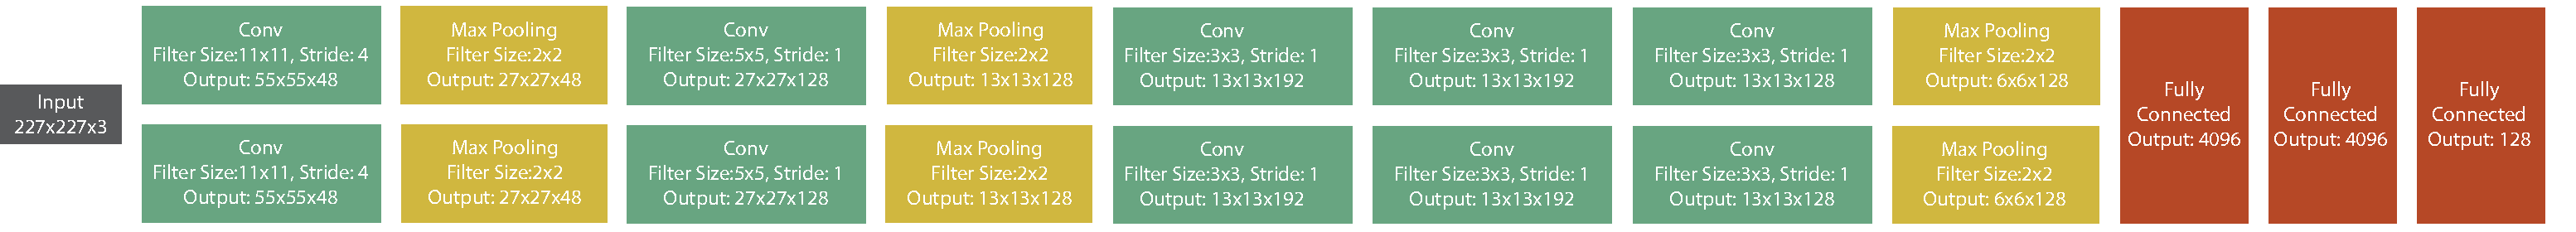
\includegraphics[width=\columnwidth]{alexnet}


where \textbf{C} is convolution, \textbf{P} is max-pooling, \textbf{R} is ReLU and \textbf{F} is fully connected layer. 

Since the office dataset is quite small, we do not learn the full network for office experiments and instead we only optimize for fully connected layers initializing with the weights pre-trained on ImageNet. Moreover, in all of our experiments, we set the feature dimension as $128$. We use stochastic gradient descent in order to learn the feature function as well as the similarity metric with AdaGrad\cite{adagrad}. We initialize all variables with truncated normals having unit variance and use the learning rate \SI{2.5e-4}  and the batch size $256$. 

We further share our learned models as well as the source code using TensorFlow\cite{tensorflow} on \url{http://anonymous.xyz}


\subsection{Evaluation Procedure}
We evaluate all algorithms in fully transductive setup following the standard evaluation setup of \cite{office}.  We feed training images and labels of the first domain as the source and feed training images of the second domain as the target. We further evaluate the accuracy on the target domain labels as the ratio of correctly labeled images to all target images. In order to evaluate our algorithm fairly, we first use cross-validation to decide on the margin $\alpha$ and label propagation tradeoff $\lambda$. 



\subsection{Results}
Following the fully transductive evaluation, we summarize the results in Table~\ref{tab:res} and Table~\ref{tab:res2}. Table~\ref{tab:res} summarizes the experimental results on the object recognition experiment using office dataset whereas  table~\ref{tab:res2} summarizes the digit classification experiments on MNIST and SVHN.

Table~\ref{tab:res} suggests that our algorithm is on-par with the state of the art methods for D-SLR$\leftrightarrow$Webcam experiments. This is rather expected since the domain difference is very minor between D-SLR and webcam images and the minor domain difference results in saturation of accuracies for all algorithms. Moreover, since we use nearest neighbor classifier, our algorithm needs a large-dataset to be successful. Both webcam and D-SLR datasets are rather small (300to700 examples) which limits the accuracy of nearest neighbor algorithm as well.

Table~\ref{tab:res} further suggests our algorithm significantly outperforms all state-of-the-art methods when there is a large domain difference like MNIST$\leftrightarrow$MNIST-M, MNIST$\leftrightarrow$SVHN, Amazon$\leftrightarrow$Webcam and Amazon$\leftrightarrow$D-SLR. We hypothesize this performance is because of the transductive modeling. State-of-the-art algorithms like \cite{ganin15} are seeking for set of features invariant to the domains whereas we are seeking for an eplicit similarity metric explaining both differences and similarities of domains. In other words, instead of seeking for an invariance, we seek for an equivariance.

Another interesting conclusion is the asymmetric nature of the accuracy results. For example, the accuracy of adapting webcam images to amazon images and adapting amazon images to webcam images is significantly different. The similar behavior exist in MNIST and SVHN domains as well. This observation validates the importance of an asymmetric modeling and the limited performance of domain invariance based methods since they are symmetric by definition. 

\begin{figure}[ht]
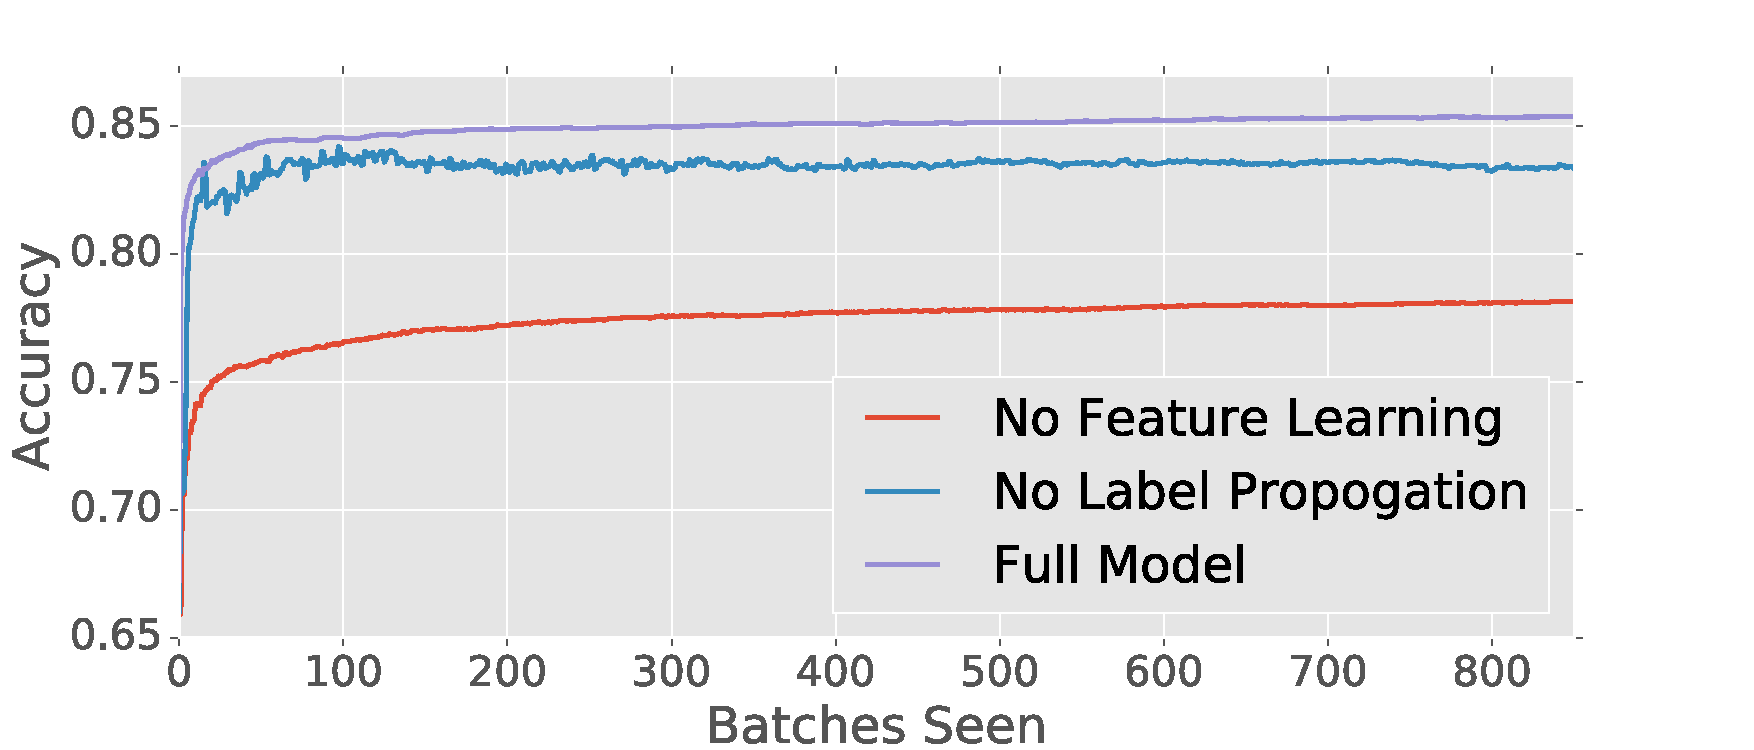
\includegraphics[width=\columnwidth]{no_feature_propogation}
\caption{Accuracy vs number of iterations for our-method and its variant without label propagation as well as the variant without feature learning. As the figure suggests the label propagation both increase the stability of the gradients as well as the final accuracy. Moreover, the feature learning also have a significant effect on the accuracy.}
\label{fllprop}
\end{figure}

\subsubsection{Qualitative Analysis}
To further study the learned representations as well as the similarity metric, we perform a series of qualitative analysis in the form of nearest neighbor analysis and tSNE\cite{tsne} plots.

In Figure~\ref{fig:nn}, we visualize example target images from MNIST and their corresponding source images. First of all, both our experimental procedure and qualitative analysis suggests that MNIST and SVHN are the two domains with largest difference. Hence, we believe MNIST$\leftrightarrow$ is very challenging set-up. Moreover, our algorithm results in very accurate nearest neighbors.

In Figure~\ref{fig:nnoffice},  we visualize example target images from webcam and their corresponding nearest source images from Amazon. The accuracy of the domain adaptation is also visible in this task. Please also note that the accuracy significantly degrades after the first few nearest neighbor which is also expected since we are only enforcing nearest datapoint to have the same label.

\begin{figure}[ht]
\begin{small}
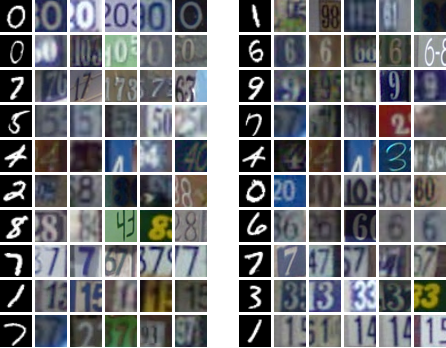
\includegraphics[width=\columnwidth]{digit_nn.png}
\vspace{-5mm}
\caption{Example nearest neighbors for SVHN$\rightarrow$MNIST experiment. We show an example MNIST image and 5-NN SVHN images. Please note the large domain difference.}
\label{fig:nn}
%\end{figure}
%\begin{figure}[ht]
\includegraphics[width=\columnwidth]{nnfi-01.png}
\caption{Example nearest neighbors for Amazon$\leftrightarrow$Webcam experiment. We show an example source image and 3-NN target images. The drop of the accuracy after the nearest neighbors is expected since our loss function only models the nearest one.}
\label{fig:nnoffice}
\end{small}
\end{figure}

The difference between invariance and equivariance is more clear in the tSNE plots of the office dataset in Figure~\ref{fig:tsne} as well as digit classification task Figure~\ref{fig:tsnedigit}. We plot same distribution twice with different color codings in Figure~\ref{fig:tsne}. In the first row, we color code each class both in source and target domains as well as before and after adaptation. As the first row of the figure suggests, the source domain is well clustered according to the object classes with and without adaptation. Moreover, this is expected since the features are specifically fine-tuned to the source domain before the adaptation starts. However, target domain has no structure. This is also expected since the algorithm did not see any image from the target domain. After the adaptation, target images also gets clustered according to the object classes. This discriminative features only arises because of the transductive modeling. In comparison, state of the art domain invariance based algorithms only try to be invariant to the domains without explicit modeling of discriminativeness on the target domain. Hence, out similarity metric explicitly models the relationship between the domains and results in equivariant model. We also draw lines between the nearest neighbor images of source and target images in order to show this consistent metric function. In Figure~\ref{fig:tsnedigit}, we also draw the images as well as the nearest neighbors between source and target. We see the discriminative behavior more distinctly in the digit classification experiment. The nearest neighbors are also quite accurate conforming the quantitative analysis. 



\subsubsection{Label propagation \& feature learning}
In order to evaluate the effect of having a robust label propagation and feature learning, we compare our method with a variant without the label propagation (noted as \emph{No Label Propogation}) and a variant without feature learning (noted as \emph{Ne Feature Learning}). We plot the transductive accuracy vs number of iterations in order to evaluate both the effect on learning rate as well as the resultant accuracy. Although we plot the results only for MNIST$\rightarrow$MNIST-M, the other experiments have similar results and not displayed for the sake of clarity. 

Results are shown in the Figure~\ref{fllprop}, and it suggests that both feature learning and label propagation is crucial for successful transduction. Another interesting observation is the unstable behavior when we disable label propagation. Moreover, this is also expected since without label propagation, labeling stage will have more mis-classifications and they will decrease the accuracy of the metric function..

\begin{figure*}[ht]
   \vspace{-2mm}
    \begin{subfigure}[b]{0.25\textwidth}
        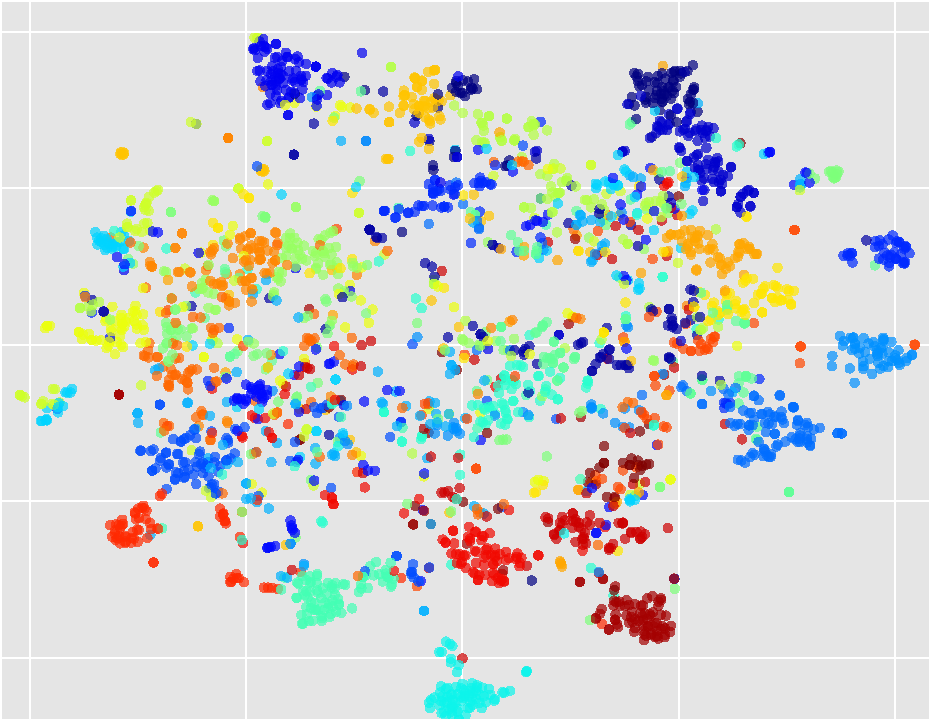
\includegraphics[width=\textwidth]{before_c_s_c}
        \caption{S. w/o Adaptation}
        \label{fig:gull}
    \end{subfigure}~\begin{subfigure}[b]{0.25\textwidth}
        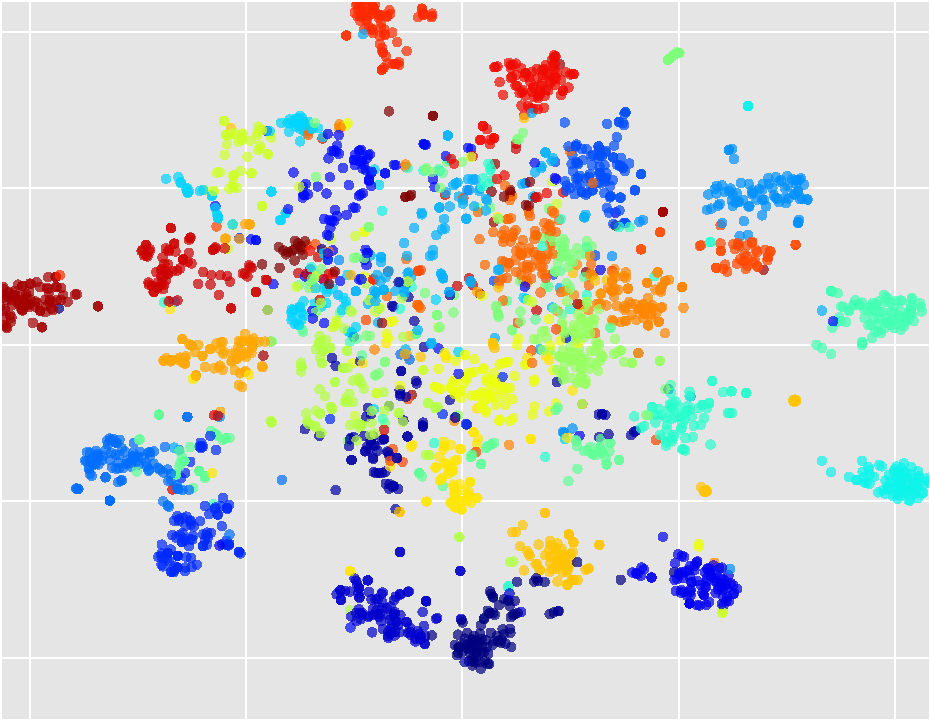
\includegraphics[width=\textwidth]{after_c_s_c}
        \caption{S. with Adaptation}
    \end{subfigure}~\begin{subfigure}[b]{0.25\textwidth}
        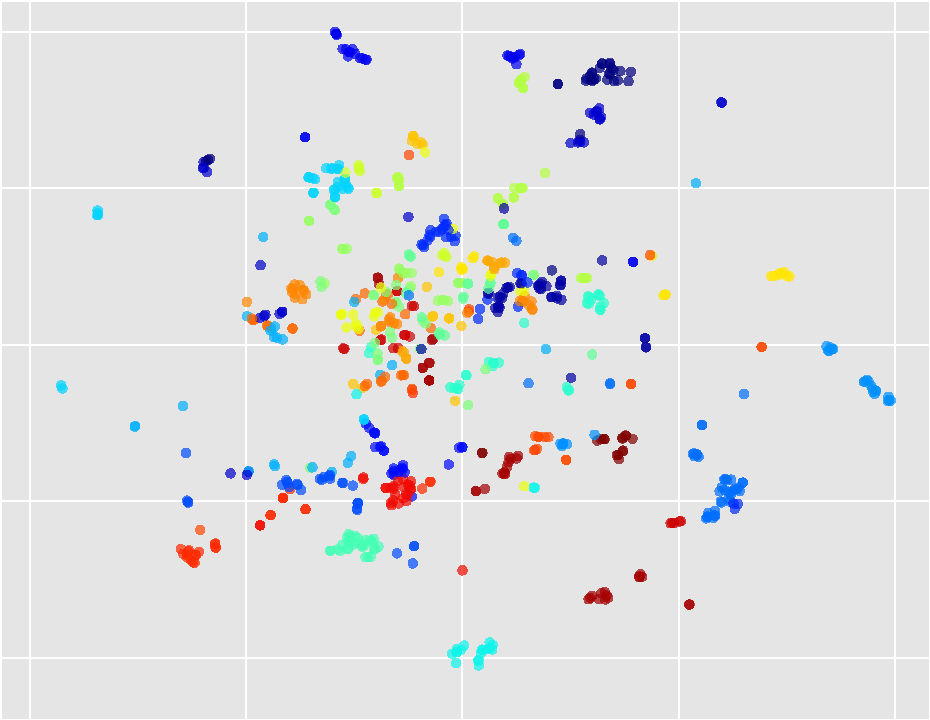
\includegraphics[width=\textwidth]{before_c_t_c}
        \caption{T w/o Adaptation}
        \label{fig:gull}
    \end{subfigure}~\begin{subfigure}[b]{0.25\textwidth}
        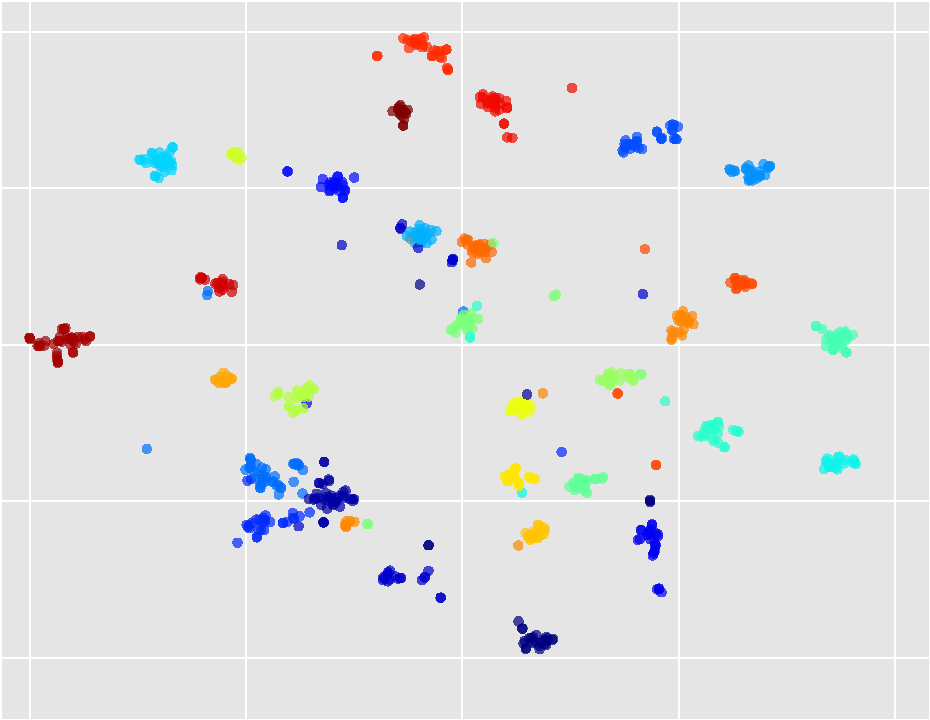
\includegraphics[width=\textwidth]{after_c_t_c}
        \caption{T with Adaptation}
    \end{subfigure}
    \vspace{-5mm}
    \caption{tSNE plots for office dataset Webcam$\rightarrow$Amazon. Source features were discriminative and stayed discriminative as expected. On the other hand, target features became quite discriminative after the adaptation.}
    \label{fig:tsne}
    \begin{subfigure}[b]{\textwidth}
        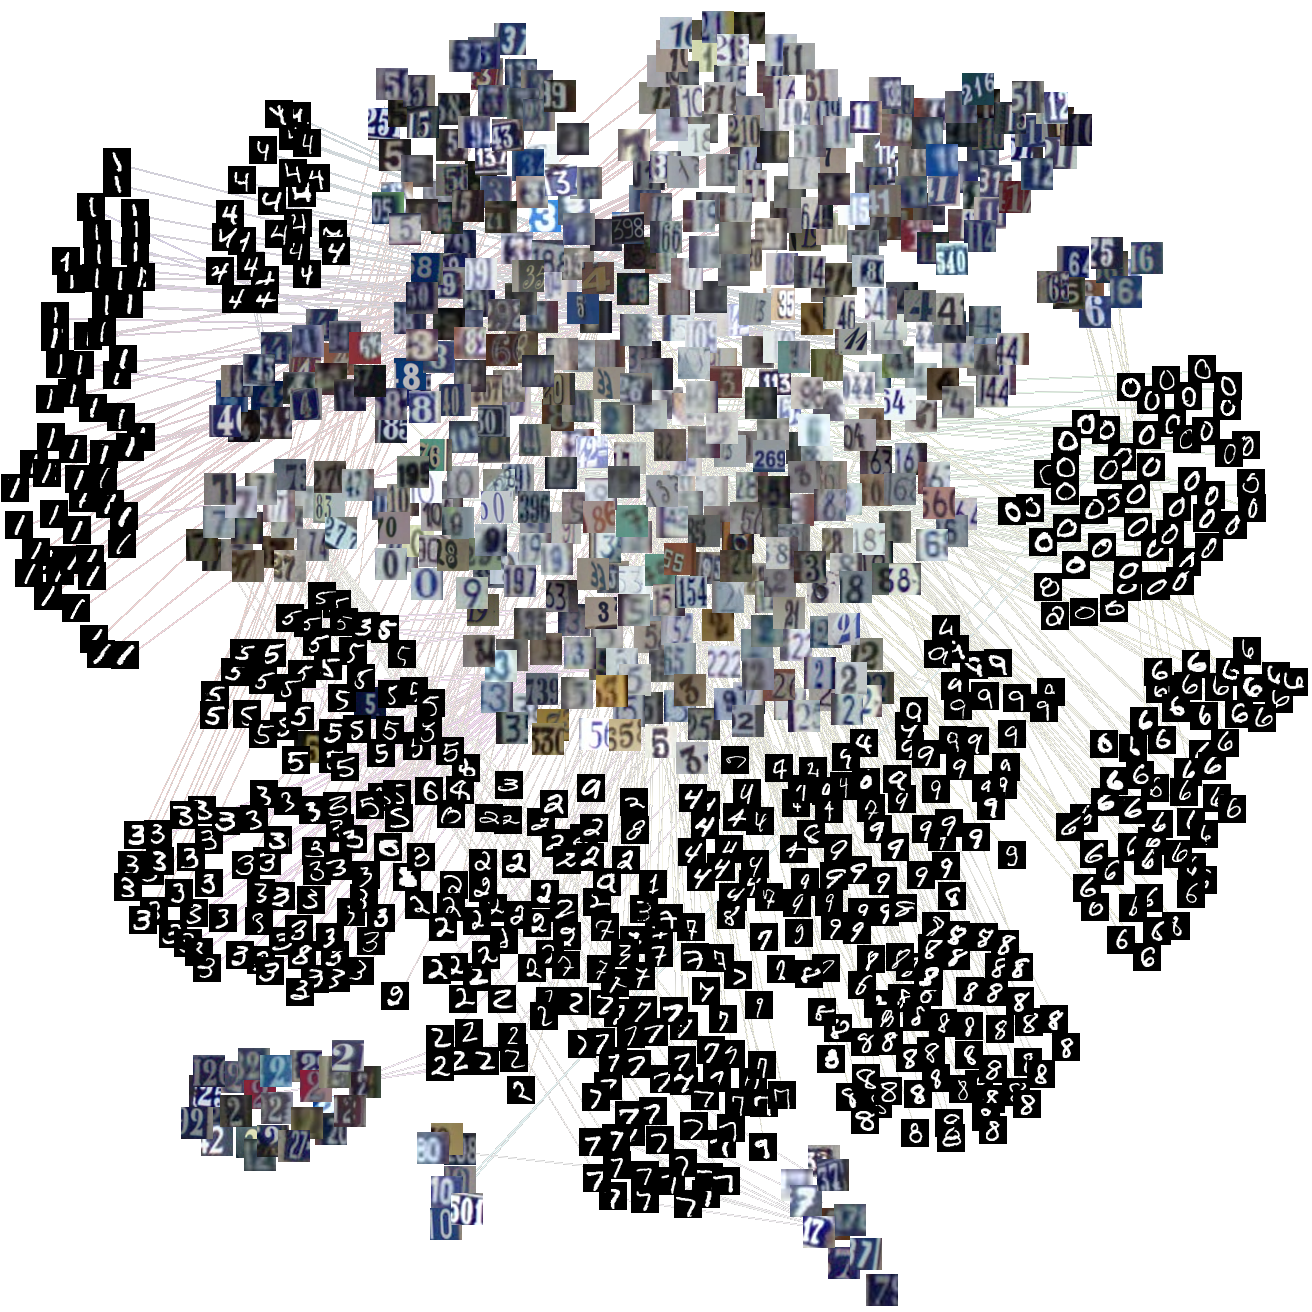
\includegraphics[width=\textwidth]{out_im.png}
        \vspace{-5mm}
        \caption{SVHN $\rightarrow$ MNIST Embeddings}
        \label{fig:tsnedigit}
    \end{subfigure}
    
\caption{tSNE plot for SVHN$\rightarrow$MNIST experiment. Please note that the discriminative behavior only emerges in the unsupervised target instead of source domain. This explain the motivation behind modeling the problem as transduction. In other words, our algorithm is designed to be accurate and discriminative in the target domain which is the domain we are interested in.  }
\label{fig:tsne}
\end{figure*}

\section{Conclusion} 
%Curabitur tincidunt urna arcu, a rhoncus lorem accumsan ac. Sed in congue massa. Proin pretium, quam a pellentesque consectetur, nulla enim facilisis nunc, a auctor libero elit non sem. Nullam accumsan dui at aliquam interdum. Lorem ipsum dolor sit amet, consectetur adipiscing elit. Curabitur sed mi sed metus dapibus consequat. Sed quis eros ut magna tempus feugiat. Curabitur feugiat diam nec eleifend ultrices.



\clearpage
\bibliography{domain_transduction}
\bibliographystyle{icml2016}

\end{document} 